\documentclass[12pt]{article}
\usepackage{graphicx}
\usepackage{latexsym}
\usepackage{amssymb}
\usepackage{amsbsy}

\oddsidemargin -0.75in
\textheight 10.5in
\textwidth 7.5in
\topmargin -0.5in

\pagestyle{empty}

\def\nn{\noindent}
\def\ds{\displaystyle}

\begin{document}
\nn {\it MATH 560-01} \hfill NAME {\underline{\ \ \ \ \ \ \ \ \ \ \ \ \ \ \ \ \ \ \ \ \ \ \ \ \ \ \ \ \ \ \ \ \ \ \ \ \ \ \ \ \ \ }}

\vskip 5mm

\nn {\bf PRACTICE EXAM 1 \#2: 2:30pm--3:45am March --, 20--. (100 points)} The exam is open book, open notes, and students are permitted to use a calculator and/or computer.  Students are expected to complete the exam individually and are not permitted to communicate in any format with others during the exam.  It is advised that students show all work and attempt each question to maximize the score.
 
\vskip 5mm
%S12 E1#5
%Answer: (a) .3 (b) .8 (c) .38 (d) .5904
\nn 1. (20 points) Brand A candy comes in one of three colors: brown, green, or red.
The probability distribution for the colors of Brand A candy is shown below.
\begin{center}
 \begin{tabular}{l|ccc} \hline
  Color & Brown & Green & Red \\ \hline
  Probability & 0.5 & ? & 0.2 \\ \hline
 \end{tabular}
\end{center}
\nn (a -- 5 pts) If one piece of candy is drawn at random from a bag of Brand A candy,
what is the probability that it will be green? {\bf \underline{\ \ \ \ \ \ \ \ \ \ \ \ \ \ \ }} \\ \\
\nn (b -- 5 pts) If one piece of candy is drawn at random from a bag of Brand A candy,
what is the probability that it will not be red? {\bf \underline{\ \ \ \ \ \ \ \ \ \ \ \ \ \ \ }} \\ \\
\nn (c -- 5 pts) If two pieces of candy are drawn at random from separate bags of Brand A candy
(independently of each other), what is the probability that both will be the same color? 
{\bf \underline{\ \ \ \ \ \ \ \ \ \ \ \ \ \ \ }} \\ \\
\nn (d -- 5 pts) If four pieces of candy are drawn at random from separate bags of Brand A candy
(independently of each other), what is the probability that at least one will be red? 
{\bf \underline{\ \ \ \ \ \ \ \ \ \ \ \ \ \ \ }}
\newpage
%S12 E1#6
%Answer: (a) 10.16 (b) .0762 (c) 14 (d) .05
\nn 2. (20 points) A lamp manufacture produces a table lamp which has a base and a shade as 
illustrated below. 
\begin{center}
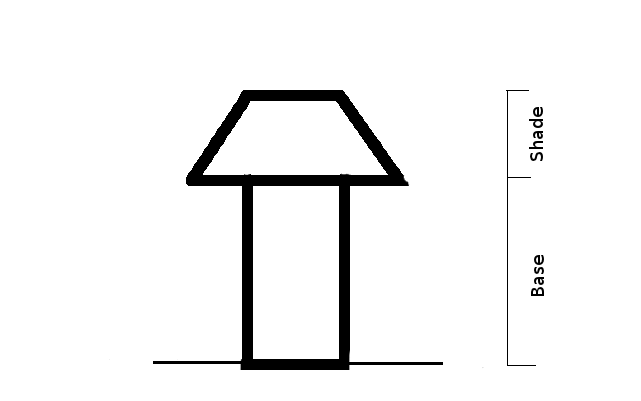
\includegraphics[height=2in]{lamp.png}
\end{center}
The height of the lamp is the sum of the height of the base and the shade.  The base and the shade are manufactured
{\bf independently}, and each varies a bit from part to part.  The heights of the bases have mean 10 inches with 
a standard deviation of 0.04 inches.  The heights of the shades have mean 4 inches with standard deviation
of 0.03 inches. \\ \\
\nn (a -- 5 pts) There are 2.54 centimeters in an inch.  What is the mean of the heights of the
shades produced by the manufacturer in centimeters? {\bf \underline{\ \ \ \ \ \ \ \ \ \ \ \ \ \ \ }} \\ \\
\nn (b -- 5 pts) What is the standard deviation of the heights of 
the shades produced by the manufacturer in centimeters? {\bf \underline{\ \ \ \ \ \ \ \ \ \ \ \ \ \ \ }} \\ \\
\nn (c -- 5 pts) What is the mean of the heights of the table lamps produced by the manufacturer in 
inches? {\bf \underline{\ \ \ \ \ \ \ \ \ \ \ \ \ \ \ }} \\ \\
\nn (d -- 5 pts) What is the standard deviation of the heights of the table lamps produced by the 
manufacturer in inches? {\bf \underline{\ \ \ \ \ \ \ \ \ \ \ \ \ \ \ }} \\ \
\newpage
%F13 Final#2
%Answer: .4207
\nn 3. (20 points) Suppose that the time between a pair of consecutive text messages arriving on a cell phone is governed by a skewed continuous distribution with mean $\mu=50$ minutes and standard deviation $\sigma=50$ minutes. 
Based on the Central Limit Theorem, what is the approximate probability that the mean time for 100 independent pairs of consecutive text messages is more than 51 minutes? {\bf \underline{\ \ \ \ \ \ \ \ \ \ \ \ \ \ \ \ \ \ \ \ \ \ \ \ \ \ \ }}
\newpage
% modified F13 Final#3
%Answer: (a) (19.943, 19.957) (b) 22
\nn 4. (20 points) To assess the accuracy of a laboratory scale, a standard weight known to weigh 20 grams is weighed repeatedly.  The scale readings are Normally distributed with unknown mean (this mean is 20 grams if the scale has no bias).  The standard deviation of the scale readings is known to be 0.01 grams. \\ 
(a -- 10 pts) A scientist collects the following 9 independent observations of scale readings, in grams:
\[
19.94, 19.96, 19.95, 19.95, 19.95, 19.95, 19.97, 19.94, 19.94.
\]
Compute a 95\% confidence interval for $\mu$.  \\ 
Round the values to at least 3 decimal places. {(\underline{\ \ \ \ \ \ \ \ \ \ \ \ \ \ \ }, \underline{\ \ \ \ \ \ \ \ \ \ \ \ \ \ \ })} \\ \\
(b -- 10 pts) Find the smallest sample size needed to have a margin of error of at most $0.005$ with 98\% confidence. {\bf \underline{\ \ \ \ \ \ \ \ \ \ \ \ \ \ \ \ \ \ \ \ \ \ \ \ \ }} 
\newpage
%S12 E2#1
%Answer: 
%Test H0: mu=110 versus Ha: mu > 110.
%The test statistic is z=2.4.
%The P-value= is 0082.
%So, we reject H0 at level .01.
\nn 5. (20 points) There is a psychological test that measures motivation, attitude towards school,
and study habits of students. The mean score for U.S.~students is 110 and the standard deviation is 20.  
A teacher who suspects that older students have better attitudes toward school gives the test to a random sample of 
16 older students.  Their mean score is $\bar{x}=122$.

Assume that the scores for the population of older students follows a normal distribution with
unknown mean $\mu$ and known standard deviation $\sigma=20$.  Should the null hypothesis 
$H_0: \mu=110$ be rejected at 
level $\alpha=.01$?  State appropriate hypotheses, calculate an appropriate test statistic, compute 
the $P$-value or critical value, and state your conclusion.
\end{document}